%!TEX root = ../thesis.tex

% https://en.wikipedia.org/wiki/Kelly_Johnson_(engineer)
% https://en.wikipedia.org/wiki/KISS_principle
\begin{savequote}[40mm]
	\textbf{K}eep\\
	\textbf{I}t\\
	\textbf{S}imple\\
	\textbf{S}tupid
	\qauthor{Kelly Johnson}
\end{savequote}

\chapter{Proposed solution}\label{chapter:proposed_solution}

	This chapter contains the technical description of ``\textit{Open LoRa Mesh}'', a mesh network composed by FiPy devices that communicate with each other via LoRa.
	Open LoRa Mesh is able to accommodate small messages, such as the ones sent by MegaSense, described in Section~\ref{subsec:megasense}.
	All network related functions are contained in a library that describes main components of this project.

	Even though it would have been possible to use a simulator, such as ``\textit{The one}''\footnote{ \url{akeranen.github.io/the-one}}, for demonstrating the usefulness of such network, the final project has been realized with Pycom hardware, discussed in Section~\ref{sec:hardware_solution}.
	
	The code created for this project is open sourced and available on GitHub under the repository \textit{Open LoRa Mesh} \footnote{ \url{www.github.com/cipz/OpenLoRaMesh}}, and better explained in the following Section~\ref{sec:software_solution}.
	
	\section{Network architecture}\label{sec:architecture}
		
		Before talking about the architecture of Open LoRa Mesh, it is important to understand the one of the MegaSense.
		As can be seen in Figure~\ref{img:megasense_architecture}, since each MegaSense device is made to be carried by a person, devices connect each one to the user's phone.
		The latter then communicates with the MegaSense and, via the application developed by the Computer Science Department at the University of Helsinki, sends the air-quality readings and the GPS location, which has been read by the application from the phone itself, to the servers in the cloud.
		
		Communication between MegaSense and phone is done via BLE, and exchanges data such as sensor readings (like NO2,
		O3, CO, battery percentage, \textit{etc.}) and calibration measurements, in \texttt{JSON} format.
		Thus each device has to be linked to a person's phone, which might enhance the portability of the device, but not its possibility to read data independently if placed in a specific location.
		Such communication resembles the one from devices described in Section~\ref{subsec:commercial_applications}.
		
		\begin{figure}[h]
			\centering
			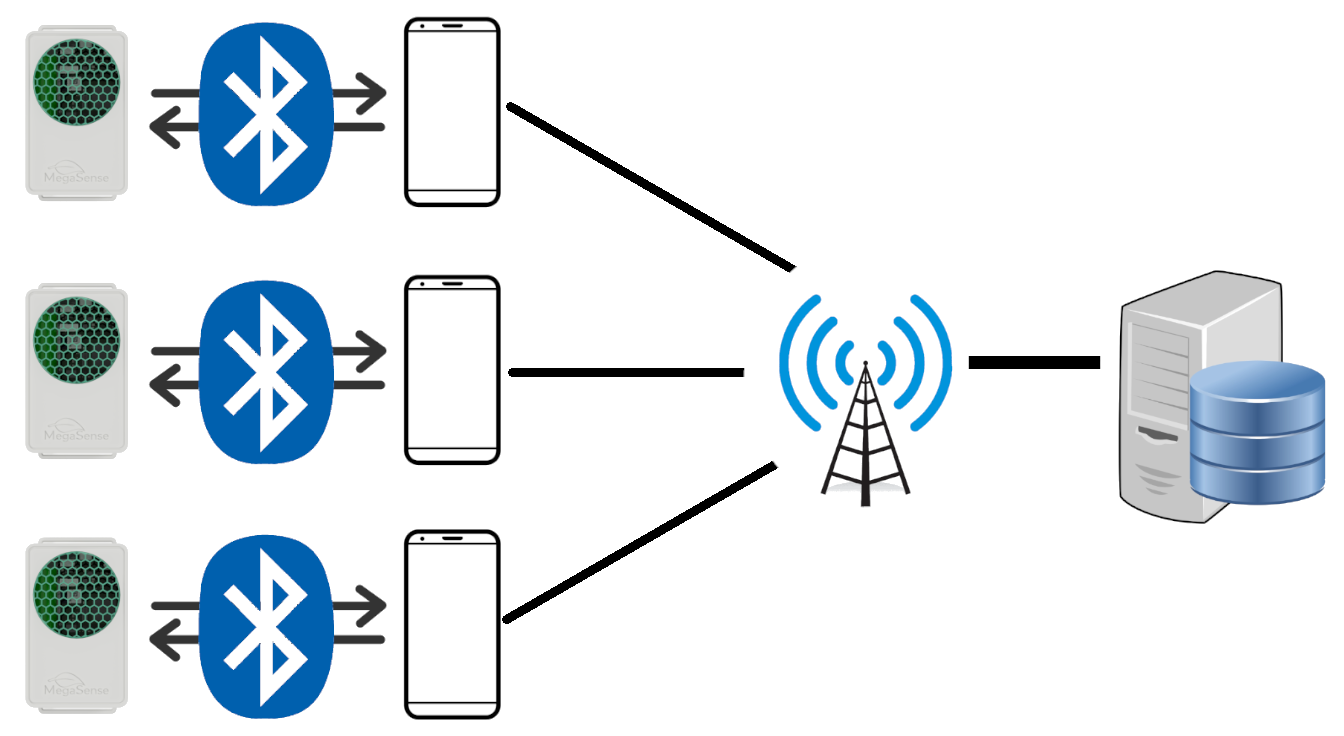
\includegraphics[width=.75\textwidth]{resources/img/chap5/architecture_megasense}
			\caption{MegaSense architecture}
			\label{img:megasense_architecture}
		\end{figure}
	
		One of the goals Open LoRa Mesh tries to achieve is to give independence to these devices so that they can communicate with one another and allow information to be passed along between nodes without the aid of a user's phone.
	
		This is why the architecture would evolve from the one in Figure~\ref{img:megasense_architecture} to Figure~\ref{img:openmesh_architecture}: the phone is replaced by a FiPy, which also connects to the MegaSense via BLE, and sends the data acquired from the sensors in the network.
		Nodes communicate with each other via LoRa, detailed in Section~\ref{subsec:lora_lorawan}, and exchange data using mainly \textit{LoRaCTP}, described in Section~\ref{subsec:loractp}.
		
		\begin{figure}[h]
			\centering
			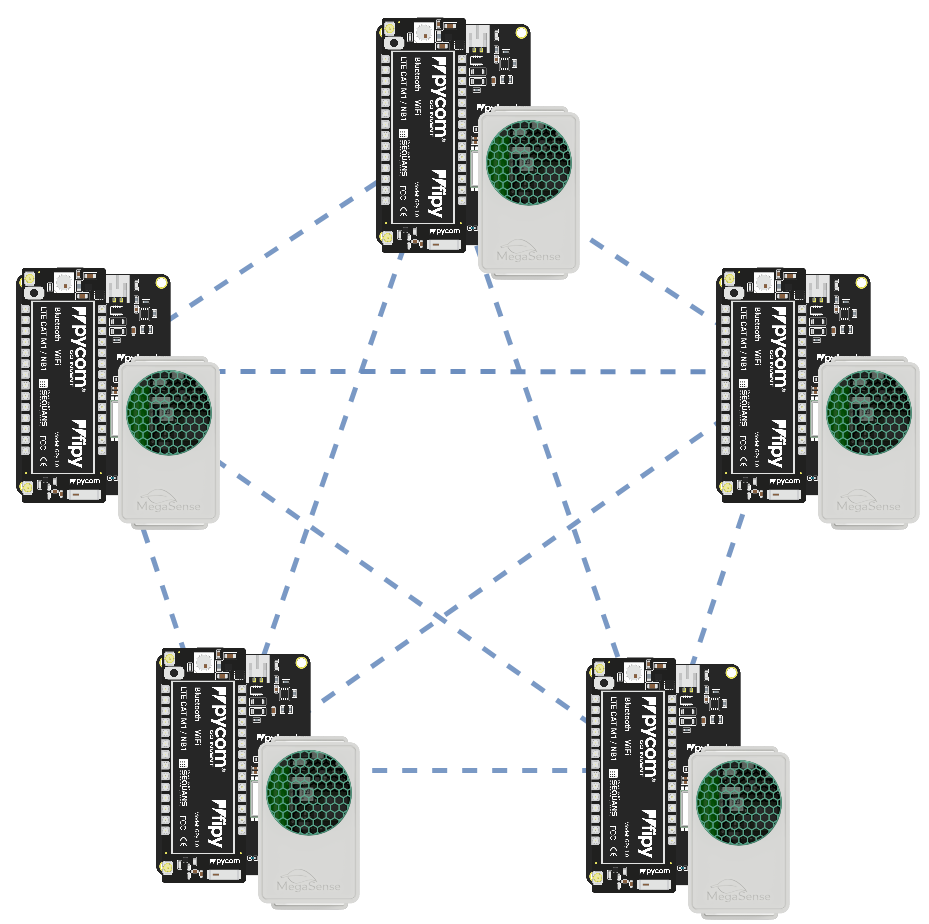
\includegraphics[width=.7\textwidth]{resources/img/chap5/mesh-architecture-1}
			\caption{Open LoRa Mesh architecture}
			\label{img:openmesh_architecture}
		\end{figure}
		
		Each FiPy board represents a node of the network, which in this case is a ``\textit{Flat Wireless Mesh}'', where each node acts both as data provider and as data forwarder.
		Although simple, such network architecture is well known from the previously mentioned, Section~\ref{sec:scalability}, Gupta and Kumar \cite{825799}.
		Besides not scaling well and having the potential to put very high resource constraints, ``\textit{addressing schemes and service discovery would prove to be a major bottleneck against scalability}'' \cite{92000412}.
		
		Despite having these disadvantages, it is important to keep in mind the small environment and the limited number of devices that will be connected in such network.
		Since communication is not frequent and data packets are not large, this network layout can satisfy the MegaSense's requirements for interconnection.

	\section{Open LoRa Mesh Hardware}\label{sec:hardware_solution}
	
		For the development of Open LoRa Mesh, the chosen hardware to replace the phone in the original MegaSense architecture is composed by Pycom's FiPy microcontrollers, along with its shields, like the PyTrack and the PySense.
		A prototype of the MegaSense device was also given from the developers of the project in order to test the connectivity with the Pycom boards and test its capacity to send and receive data from other nodes in the network.
		All devices can be seen together in Figure~\ref{img:irl_picture_1}.
		
		\begin{figure}[h]
			\centering
			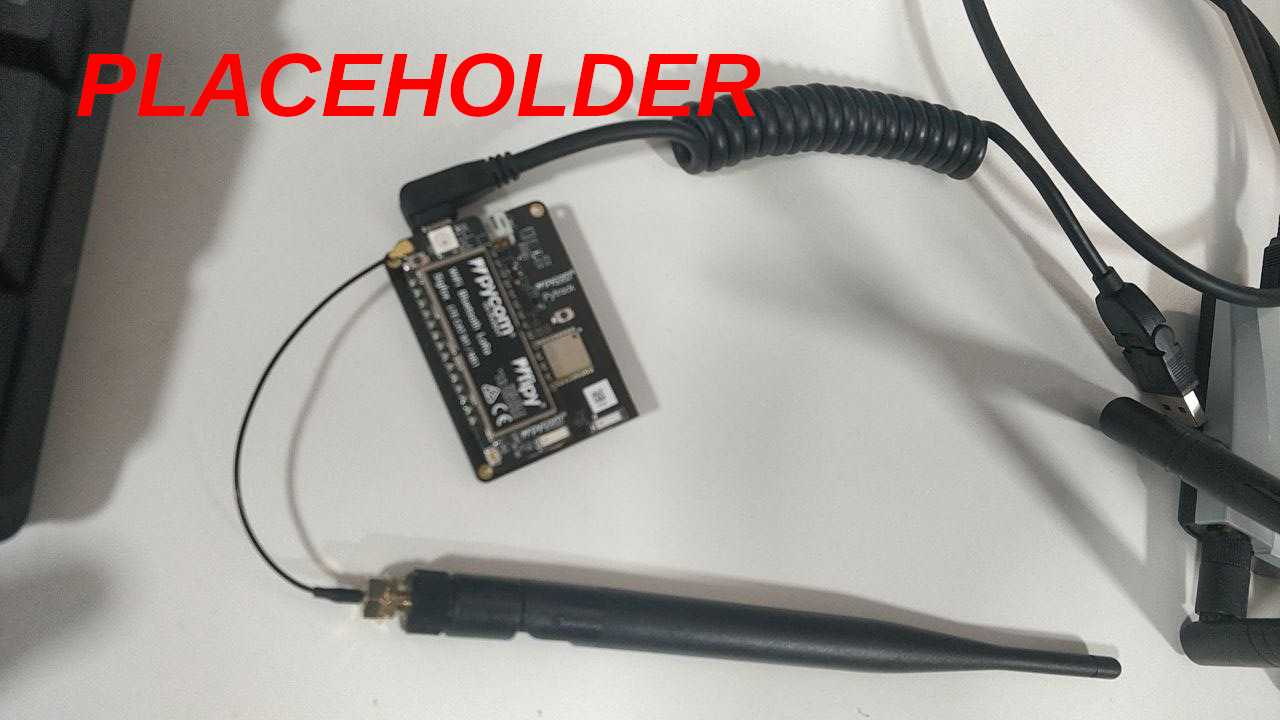
\includegraphics[width=\textwidth]{resources/img/chap5/mesh-irl-picture}
			\caption{FiPy with PyTrack, LoRa antenna, GPS antenna and MegaSense prototype}
			\label{img:irl_picture_1}
		\end{figure}
		
		Although the expansion board is important, the FiPy is the one that contains all the chips that allow connectivity, as said in Section~\ref{sec:pycom}.
		After an initial evaluation on the requirements necessary in creating a network for exchanging messages among air quality sensing devices, Pycom's boards have come first considering the numerous possibilities it allows for prototyping.
		
		The exact hardware with which this project has been completed is: four FiPy boards, one PyTrack 2X, one PyTrack, two PySense shields and one MegaSense prototype, Figure~\ref{img:megasense_picture}.
		Pycom boards do not have a USB connection directly on them, so they can be programmed either using a shield or via an UART (Universal Asynchronous Receiver-Transmitter) to USB.
		
		Alternative microcontrollers, such as the Raspberry Pi Pico, Raspberry Pi 4, Arduino Nano 33 BLE Sense, and ESP32 boards have been discard given either their excessive power or their need for multiple expansion shields.
				
	\section{Open LoRa Mesh Software}\label{sec:software_solution}
	
		While Arduino's C++ dialect divides the code in two main functions, the \texttt{setup()} and \texttt{loop()}, as mentioned in Chapter~\ref{chapter:technologies}, the Pycom boards use two files to separate an initial bootstrap of the board and a main section of the code.
		These two special files are called \texttt{boot.py} and \texttt{main.py} respectively.
		
		The following section explains the algorithms made for this project are delineated and it is shown how they have been implemented.
		Afterwards, the addressing scheme in LoRa, which is important to understand, is described.
		
		All network related functions are contained in a library that describes main components of this project.
		
		The FiPy boards have been programmed using Micropython, and the firmware flashed\footnote{ \textit{Flashing} involves the overwriting of existing firmware or data, contained in EEPROM or flash memory module present in an electronic device, with new data.} on the boards, at the time of writing, is \texttt{v1.16.5}.
		
		\subsection{Important functions}\label{subsec:algorithms}
	
			% DRAWING AUTOMATA
			% https://latexdraw.com/automata-diagrams-in-latex/
			% https://hayesall.com/blog/latex-automata/
			
			% DRAWING FLOWCHART
			% https://www.overleaf.com/learn/latex/LaTeX_Graphics_using_TikZ%3A_A_Tutorial_for_Beginners_(Part_3)%E2%80%94Creating_Flowcharts

			This subsection shows in depth how the software works, for more significant building block of the code there are finite-state automata (or FSA) that show the state nodes find themselves in.
			For a graphical reason, each state of the following automata is abbreviated, and, when needed, the full state is described in a table underneath it.
			
			At first an overview of the entire software is presented, then for each important component of the software there is a subsection that describes how it functions and connects to the rest.
			Such vision should allow to understand the system from a broader point of view to a more detailed one, where every function is analyzed.
			
			\subsubsection{Overview of the whole system}
			
				As previously said, the FiPy is divided in two files, \texttt{boot.py} and \texttt{main.py}.
				When the board is powered up, the first file executed is \texttt{boot.py}, which contains the code that either boots the device in a state of receiver or continues its normal sequence.
				
				The receiver state allows for the device to be used as a station that only sniffs the messages traveling in the air.				
				Continuing in the normal sequence, thus executing the code in \texttt{main.py}, will allow the node to connect to an existing mesh or to create one, for sending and receiving data afterwards.
				
				Open LoRa Mesh heavily relies on the use of LoRaCTP, described in Section~\ref{subsec:loractp}, for message transmission.
				This is because LoRaCTP builds an important layer of stability on top of raw LoRa transmission.
				
			\subsubsection{Boot sequence}
			
				As mentioned earlier, the \texttt{boot.py} file contains the code that is initially executed by the FiPy.
				The first operation done is to disable Wi-Fi communication and the default blinking (heartbeat) of the FiPy, Figure~\ref{code:boot_wifi}.
				Since when powered up, FiPy's firmware enables Wi-Fi, it can be useful to turn it off because it is not used, also it could draw unnecessary power from the device.

				\begin{figure}[H]
					\begin{lstlisting}[language=Python]
wlan = WLAN(mode=WLAN.STA)
wlan.deinit()
pycom.heartbeat(False)
					\end{lstlisting}
					\caption{Code for Wi-Fi de-initialization and heartbeat stop}
					\label{code:boot_wifi}
				\end{figure}
			
				During the boot procedure, the board checks the availability of a \texttt{config.json} file on an external SD card and, if present, uses the parameters on such files.
				If not present it checks for such file locally on the flash memory, which contains one with default configurations and is uploaded with the \texttt{*.py} files.

				The configuration file contains the custom parameters that can be used by the board, and
				include \texttt{BOOT\_MODE}, which can either be \texttt{DEFAULT\_BOOT} or \texttt{PLAIN\_RECEIVER}.
				If set to \texttt{DEFAULT\_BOOT}, the board will normally proceed to executing the software in \texttt{main.py}.
				When set to \texttt{PLAIN\_RECEIVER}, the board will execute code which makes it listen to the packets traveling in the air.
				Such process can be seen in Figure~\ref{fsa:boot_sequence}, described in Table~\ref{table:fsa_boot}
				
				Other modes could be added to the software as an improvement, but at the time of writing only these have been implemented.
				Improvements on this topic is later about in Section~\ref{sec:software_improvements}.
									
				\begin{figure}[h]
					\centering
					\begin{tikzpicture}[shorten >=1pt,node distance=2cm,on grid,auto]
					
					% Help grid
					% \draw [help lines] (-1,1) grid (6,-6);
					
					\tikzstyle{every state}=[fill={rgb:black,1;white,5}]
					
					
					\node[state, initial]  			(s_0)                 	{$s_0$}; % START
					\node[state] 					(s_1)	[right of=s_0]	{$s_1$}; % BOOT
					\node[state, accepting]			(s_2) 	[above right of=s_1]	{$s_2$}; % MAIN LOOP
					\node[state, accepting]			(s_3) 	[below right of=s_1]	{$s_3$}; % RECEIVER LOOP
					
					\path[->]
					(s_0) edge node {} (s_1)
					(s_1) edge node {} (s_2)
					(s_1) edge node {} (s_3)
					(s_2) edge [loop right] node {} ()
					(s_3) edge [loop right] node {} ();
					
					\end{tikzpicture}
					\caption{FSA for the overview of boot sequence}
					\label{fsa:boot_sequence}
				\end{figure}				
		
				\begin{table}[h]
					\begin{center}
						\begin{tabular}{|c|m{10.2cm}|} 
							\hline
							\textbf{State abbreviation} & \textbf{State description} \\\hline
							$start$ & device is powered up\\\hline
							$s_{0}$ & Wi-Fi is de-initialized and heartbeat is set to \texttt{False}\\\hline
							$s_{1}$ & configuration file is read\\\hline
							$s_{2}$ & \texttt{PLAIN\_RECEIVER} mode is initialized\\\hline
							$s_{3}$ & \texttt{DEFAULT\_BOOT} mode is initialized\\\hline
						\end{tabular}
						\caption{Boot sequence FSA description}
						\label{table:fsa_boot}
					\end{center}
				\end{table}

			\subsubsection{Plain receiver}
			
				The mode in which the device is set only to listen is called ``\textit{\texttt{PLAIN\_RECEIVER}}'', and the code executed is contained in the \texttt{plain\_receiver.py} file.
				Such state lets the FiPy listen to messages that are in its range, without the possibility of sending messages or participate into the mesh.
				This state can be used for debugging and catching the different messages that are sent in an area.
				
				\begin{figure}[H]
					\begin{lstlisting}[language=python]
def sniffLoRaNetwork():
  ctpc = loractp.CTPendpoint()
  print("Executing plain_receiver.py")
  while True:
    print('plainreceiver.py: waiting for data')
    try:
      rcvd_data, addr = ctpc.recvit()
      print("plainreceiver.py: got {} from {}".format(rcvd_data, addr))
    except Exception as e:
      print ("plainreceiver.py: EXCEPTION!! ", e)
					\end{lstlisting}
					\caption{\texttt{PLAIN\_RECEIVER} mode code}
					\label{code:plain_receiver}
				\end{figure}

				The principal function in the file \texttt{plain\_receiver.py} is \texttt{plain\_receiver()}, in Figure~\ref{code:plain_receiver}.
				Such function is an adaptation of the example one contained in the LoRaCTP repository.
				It first creates an endpoint, which is then used in an infinite loop that reads data received at the endpoint and logs it.
				
			\subsubsection{Main sequence and key variables}
			
				This subsection describes the course of the \texttt{main.py} file and the \texttt{main()} function it contains.
				The code contained in this file is automatically executed by the board, unless specified otherwise, after the code in the previously described \texttt{boot.py} file.
				
				\begin{figure}[h]
					\centering
					\begin{tikzpicture}[shorten >=1pt,node distance=2cm,on grid,auto]
					
					% Help grid
					% \draw [help lines] (-1,1) grid (6,-6);
					
					\tikzstyle{every state}=[fill={rgb:black,1;white,5}]
					
					
					\node[state]  					(s_3)                 	{$s_3$}; % PICKS UP FROM BOOT
					\node[state] 					(m_0)	[right of=s_3]	{$m_0$}; % INITIALIZE VARIABLES AND OBJECTS AND LOCKS THE LORA ANTENNA AND CREATES CONNECTION WITH MEGASENSE, IF AVAILABLE
					\node[state]					(m_1) 	[right of=m_0]	{$m_1$}; % LISTEN LOOP FOR MESSAGES OF EXISTING LORA MESHES
					\node[state]					(m_2) 	[above right of=m_1]	{$m_2$}; % LORA MESH EXISTS
					\node[state]					(m_3) 	[below right of=m_1]	{$m_3$}; % LORA MESH DOES NOT EXIST, CREATE NEW MESH
					\node[state,accepting]			(m_4) 	[above right of=m_3]	{$m_4$}; % NODE LISTENS FOR MESSAGES IN THE AIR AND ANALYZES IT
					\node[state]					(m_5) 	[right of=m_4]	{$m_5$}; % IF AVAILABLE COMMUNICATES WITH MEGASENSE AND READS DATA FROM IT
					\node[state]					(m_6) 	[right of=m_5]	{$m_6$}; % COMMUNICATE WITH MEGASENSE
					
					\path[->]
					(s_3) edge node {} (m_0)
					(m_0) edge node {} (m_1)
					(m_1) edge [loop above] node {} ()
					(m_1) edge node {} (m_2)
					(m_1) edge node {} (m_3)
					(m_3) edge node {} (m_4)
					(m_2) edge node {} (m_4)
					(m_4) edge node {} (m_5)
					(m_5) edge node {} (m_6)
					(m_6) edge [bend left] node {} (m_4);
					
					\end{tikzpicture}
					\caption{FSA for the overview of the main code}
					\label{fsa:main}
				\end{figure}		
			
				\begin{table}[h]
					\begin{center}
						\begin{tabular}{|c|m{10.2cm}|} 
							\hline
							\textbf{State abbreviation} & \textbf{State description} \\\hline
							$s_{3}$ & state $s_{3}$ from Figure~\ref{fsa:boot_sequence} where the code \texttt{main.py} starts\\\hline
							$m_{0}$ & variables,objects and communication with MegaSense device, if available, are initialized\\\hline
							$m_{1}$ & listen loop for messages for existing LoRa mesh network\\\hline
							$m_{2}$ & if the mesh exists, the node exchanges information about it with the advertising node\\\hline
							$m_{3}$ & if the mesh does not exist, the node creates a new mesh and advertises the mesh information\\\hline
							$m_{4}$ & the node listens for any messages in the air and processes them\\\hline
							$m_{5}$ & if the MegaSense device is available, the node connects to it, reads data, and sends it into the network\\\hline
							$m_{6}$ & the node broadcasts a message advertising the mesh network\\\hline
						\end{tabular}
						\caption{Main sequence FSA description}
						\label{table:fsa_main}
					\end{center}
				\end{table}
			
				The most important objects used in the main part of this software, and that are initialized at the beginning, are:
				\begin{itemize}
					\item \texttt{LORA\_ANTENNA\_LOCK}: a \texttt{LOCK} is placed on the use of the LoRa antenna so that it can be used only in one part of the program at the time; 
				    \item \texttt{node}: represents the current node and its properties;
					\item \texttt{mesh}: contains the data about the mesh network;
					\item \texttt{routing\_table}: contains data about the other nodes connected to the mesh.
				\end{itemize}
			
				\texttt{node}, \texttt{mesh} and \texttt{routing\_table} are all objects initialized from the \texttt{mesh.py} library, later described in Section~\ref{subsec:mesh_library}.
				
				Like in the \texttt{boot()} function, \texttt{main()} also searches for a configuration file, at first on an SD card, then on the flash memory.
				Important entries in this \texttt{JSON} file used by \texttt{main()} are:
				\begin{itemize}
					\item \texttt{GPS}: a boolean that tells the FiPy to either find or not the GPS coordinates of the board. This only happens if the board is connected to a PyTrack shield;
					\item \texttt{MEGASENSE\_CONNECT}: another boolean that tells the board either to connect or not to a MegaSense device, of which the MAC address is contained in \texttt{MEGASENSE\_ADDR};
					\item \texttt{MEGASENSE\_ADDR}: address of the MegaSense device the board will connect to.
				\end{itemize}
			
				The functions related to the communication with the MegaSense device are contained in the \texttt{megasense.py} file, described in Section~\ref{subsec:megasense_lib}.
				
			\subsubsection{Mesh initialization}
			
				As can be seen in the Figure~\ref{fsa:main}, after initializing the necessary variables and objects in $ m_0 $ , the node listens for any messages that advertise an existing mesh, represented by state $ m_1 $.
				Particularly, this is done via the code in Figure~\ref{code:mesh_init_1}.
				An important thing to keep in mind when working with devices that communicate wirelessly is the channel availability.
				The node listens for \textit{at least} 180 seconds: the function \texttt{listen\_for\_mesh} of the \texttt{Node} object contains a line of code that adds a random amount of time so that nodes which start at the same time, do not overlap and cause the creation two separate mesh networks.
				
				\begin{figure}[H]
					\begin{lstlisting}
mesh_id, advertising_node, request_connection = node.listenForMesh(180)
					\end{lstlisting}		
					\caption{Code that listens for mesh network advertisements}
					\label{code:mesh_init_1}
				\end{figure}
			
				The \texttt{node.listen\_for\_mesh()} function is invoked on the \texttt{Node} object from the library in \texttt{mesh.py}, better explained later in Section~\ref{subsec:mesh_library}.				
				\texttt{request\_connection}, in Figure~\ref{code:mesh_init_1}, is a boolean variable that tells if a message has been received.
				
				If positive, the receiving node sends a request for such mesh information to the sending node, this will send the data, which includes the routing table, the routing table version and the mesh id.
				Otherwise, the current node will create a new mesh network, thus initializing the routing table with itself as parent and using the mesh id given in the configuration file.
				Such code is present in Figure~\ref{code:mesh_init_2} and represents respectively states $m_{2}$ and $m_{4}$ from Figure~\ref{fsa:main}.
									
				\begin{figure}	
					\begin{lstlisting}
if request_connection:
  mesh = Mesh(mesh_id)
  mesh_info = node.requestMeshInfo(mesh_id, advertising_node)
  mesh_info = json.loads(mesh_info.decode())

  received_routing_table_content = mesh_info["CURR_ROUTING_TABLE_CONTENT"]
  received_routing_table_version = mesh_info["CURR_ROUTING_TABLE_VERSION"]
  
  routing_table = RoutingTable(
    received_routing_table_content, 
    received_routing_table_version
  )
else:
  mesh = Mesh(force_new_mesh_id = b"OPENMESH")
  new_routing_table_dict = { node.LORA_MAC : "" }
  routing_table = RoutingTable(new_routing_table_dict)
					\end{lstlisting}
					\caption{Code use to initialize the mesh network by requesting data from the advertising node or creating a new mesh}
					\label{code:mesh_init_2}
				\end{figure}
			
%				\begin{figure}[h]
%					\centering
%					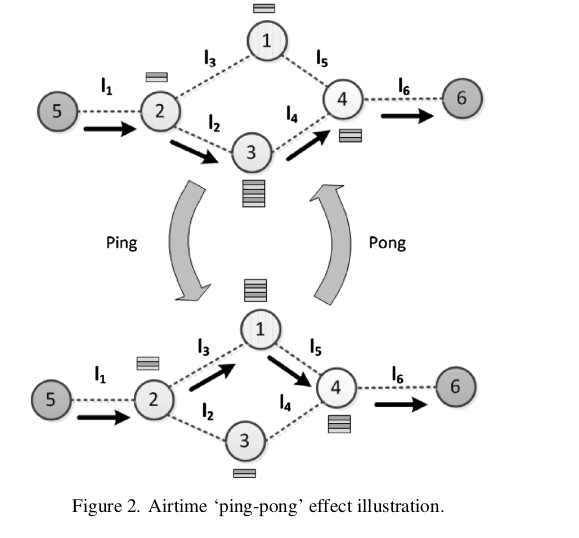
\includegraphics[width=.7\textwidth]{resources/img/chap5/message_exchange}
%					\caption{Message exchange for mesh network advertisement}
%					\label{img:message_exchange}
%				\end{figure}
	
			\subsubsection{Main loop}\label{subsec:loop}
	
				After the code in Figure~\ref{code:mesh_init_2} is executed, the code contains an infinite \texttt{while True} loop.
				Unlike the Arduino, which has the \texttt{loop()} function that runs infinitely unless ordered differently, Pycom devices only execute the contents of \texttt{main.py} once. 
				That is why this infinite loop is needed.
				
				In the FSA in Figure~\ref{fsa:main}, state $ m_{4} $ coincides with this loop.
				It is marked as an accepting state since the program might finish due to possible Exceptions.
				Such Exceptions are part of the ones described later in Section~\ref{sec:software_improvements}.
				
				At each start of the loop, \texttt{LORA\_ANTENNA\_LOCK} is acquired, thus allowing the node to send and receive data.
				This infinite loop can be divided in three parts, which are respectively states $ m_4 $, $ m_5 $ and $ m_6 $ in Figure~\ref{fsa:main}:
				% TODO COMPLETE
				\begin{itemize}
					\item $ m_4 $, listen and for incoming messages and send responses:
					\item $ m_5 $, connection with MegaSense and data gathering:
					\item $ m_6 $, broadcasting mesh advertisement:
						\begin{figure}[H]
							\begin{lstlisting}
node.broadcastMeshAdvertisement(mesh.MESH_ID)
							\end{lstlisting}
							\caption{Code for mesh advertisement in \texttt{main.py} loop}
							\label{code:mesh_advertisement_main}
						\end{figure}
					
						\begin{figure}
							\begin{lstlisting}
def broadcastMeshAdvertisement(self, mesh_id):
  msg = self.MESH_ADVERTISE_PREAMBLE.decode() + 
    "=" + mesh_id.decode() + "." + self.LORA_MAC.decode()
  self.broadcast(msg)
							\end{lstlisting}
							\caption{Code for broadcasting advertisement messages in mesh library}
							\label{code:mesh_advertisement_library}
						\end{figure}
				\end{itemize}	
			
			\subsubsection{Message forwarding}
			
				\textbf{\textcolor{red}{\hl{// To be completed}}}
			
			\subsubsection{MegaSense communication}
			
				If the boolean variable \texttt{MEGASENSE\_CONNECT} in the configuration file is set to \texttt{True}, then at the beginning of \texttt{main()} a \texttt{MegaSense} object is created.
				Such object is implemented in the \texttt{megasense.py} file, a library that contains the functions used to interact with the device.
				
				The architecture of Open LoRa Mesh implies that each node of the network communicates with a MegaSense device via BLE.
				Thus, the configuration file of each node contains \texttt{MEGASENSE\_ADDR} variable, a string with the MAC address of a specific MegaSense.
				If such sensor is in reach, then the node will connect to it and interact, gathering data about air quality in its surroundings.
				Such interaction is done via the functions in the MegaSense class, described in Section~\ref{subsec:megasense_lib}.
				
		\subsection{Mesh library}\label{subsec:mesh_library}
		
				\textbf{\textcolor{red}{\hl{// To be completed}}}
%			\subsection{Node initialization}
%				\begin{figure}
%					\begin{lstlisting}
%def __init__(self) -> None:
%  self.LORA_NETWORK = LoRa(mode=LoRa.LORA, region=LoRa.EU868)
%  self.LORA_SOCKET = socket.socket(socket.AF_LORA, socket.SOCK_RAW)
%  self.LORA_MAC = binascii.hexlify(LoRa().mac())[8:]
%  self.NODE_ID = 0x01
%					\end{lstlisting}
%					\label{code:node_initialization}
%					\caption{Code for node initialization in mesh library}
%				\end{figure}
		
%			\subsubsection{Routing table}\label{subsec:routing_table}
		
%		\subsection{LoRaCTP forwarding}\label{subsec:loractp_mesh}
		
			% spiegare come si modifica loractp
		
%		\subsection{Supported messages}
		
%	\section{LoRa addressing scheme}\label{subsec:lora_addressing}
		
		% Hardware Addressing Schemes
		
		
		%calcolare transmission times
		
%	\section{Other files}
%	
%		Figure~\ref{img:files} shows a list of all files that contribute to this project.
%		
%		\begin{figure}[h]
%			\centering
%			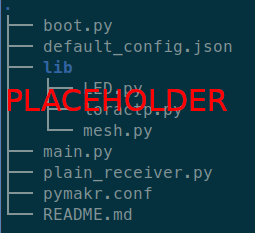
\includegraphics[width=.5\textwidth]{resources/img/chap5/tree_files}
%			\caption{List of files that compose the Open LoRa Mesh project}
%			\label{img:files}
%		\end{figure}
%	
%		\texttt{LED.py} is an LED library that allows the definition of threads in which LED functions are controlled.
%		These are used in the software and have not been explained in the previous sections since their use is secondary compared to the other functions.
%		% TODO CAMBIARE SE NECESSARIO
%		\texttt{README.md} and \texttt{banner.png} files are used in the GitHub repository and not essential to the usability of this project.

		\subsection{MegaSense library}\label{subsec:megasense_lib}
		
	\section{Microcontroller sleep cycle}\label{sec:sleep}
	
		Most IoT devices that compose LPWANs have three main modes, or profiles: \textit{sense}, \textit{connect} and \textit{sleep}.
		Sense and connect refer respectively to gathering data from the sensors and sending it into the network, while sleep refers to a sleep-mode energy consumption where most processes in the device are halted, and some circuits may be powered down.
		It can be considered a design trade-off between functionality, size, and battery lifetime.
		
		This energy consumption profile is important because it helps maximizing the battery life, which currently is one of the most considerable bottlenecks in IoT low-power devices, as explained in Section~\ref{sec:trends}.
		
		However, in the implementation of the Open LoRa Mesh, nodes do not have such functionality implemented, since might it be the cause for network disruptions.
		
		For example, if a new node might want to join a network, but the nearest physical node is in sleep mode, there would be no possibility for the new node to request data about the network, thus wasting time and resources while waiting to the other node to come back online.
		
		Such mode could be implemented but would require an careful analysis on the evolution of the network in time, also would require a network made entirely, or mostly of static nodes.
		This thought is reviewed again in Section~\ref{sec:software_improvements}.
			
	\section{Use cases}
		
		Each network topology is better suited for particular scenarios, and it is not possible to have a ``\textit{one size fits all}'' network.
		Which is why the final section of this chapter explains where Open LoRa Mesh is better suited and where it will not perform as well.
		
		\subsection{Mobile network}
		
			Mobile networks, such as bike sharing and other shared transportation environment, require high speed for adjusting. 
			These are dynamic environments where speed is important, especially for messages exchanged in the control plane, as explained for VANETs in Section~\ref{sec:overview_wms}.
			
			Open LoRa Mesh would not be well suited for such type of networks, this is because the ``\textit{raw maximum data rate of 27 kbps}'' \cite{8030482} and, when moving at high speed, devices can become very sensitive to Doppler effect \cite{s21124049}.
		
		\subsection{Fixed network}\label{sec:fixed_network}
		
			This is the type of network Open LoRa Mesh is better suited in.
			Although MegaSense works with mobile sensors, Open LoRa Mesh would allow it to work with monitoring sensors spread in a defined area.
			This could either be inside or outside a a building.
			
			Such type of network works best since it is mostly static and connections are rarely broken, thus data that needs to be sent in the control plane does not exceed the one sent in the data plane, as it can happen in the previous scenario.
		
		\subsection{Hybrid network}
		
			Such scenario includes, for example, the integration of mobile sensors given to users with a network of fixed sensors in an area.
			In this case, the usability of Open LoRa Mesh depends on the number of mobile devices that need connectivity and how many times they connect and disconnect.
			